\section{Domain Model}\label{section:domain-model}

This section presents the entities of the problem domain as well as the relationships among them. Figure~\ref{figure:domain-model1} depicts the application's domain model in the form of a \gls{uml} class diagram. The diagram does not contain all attributes but is limited to the most relevant ones.

\begin{figure}[ht]
\centering
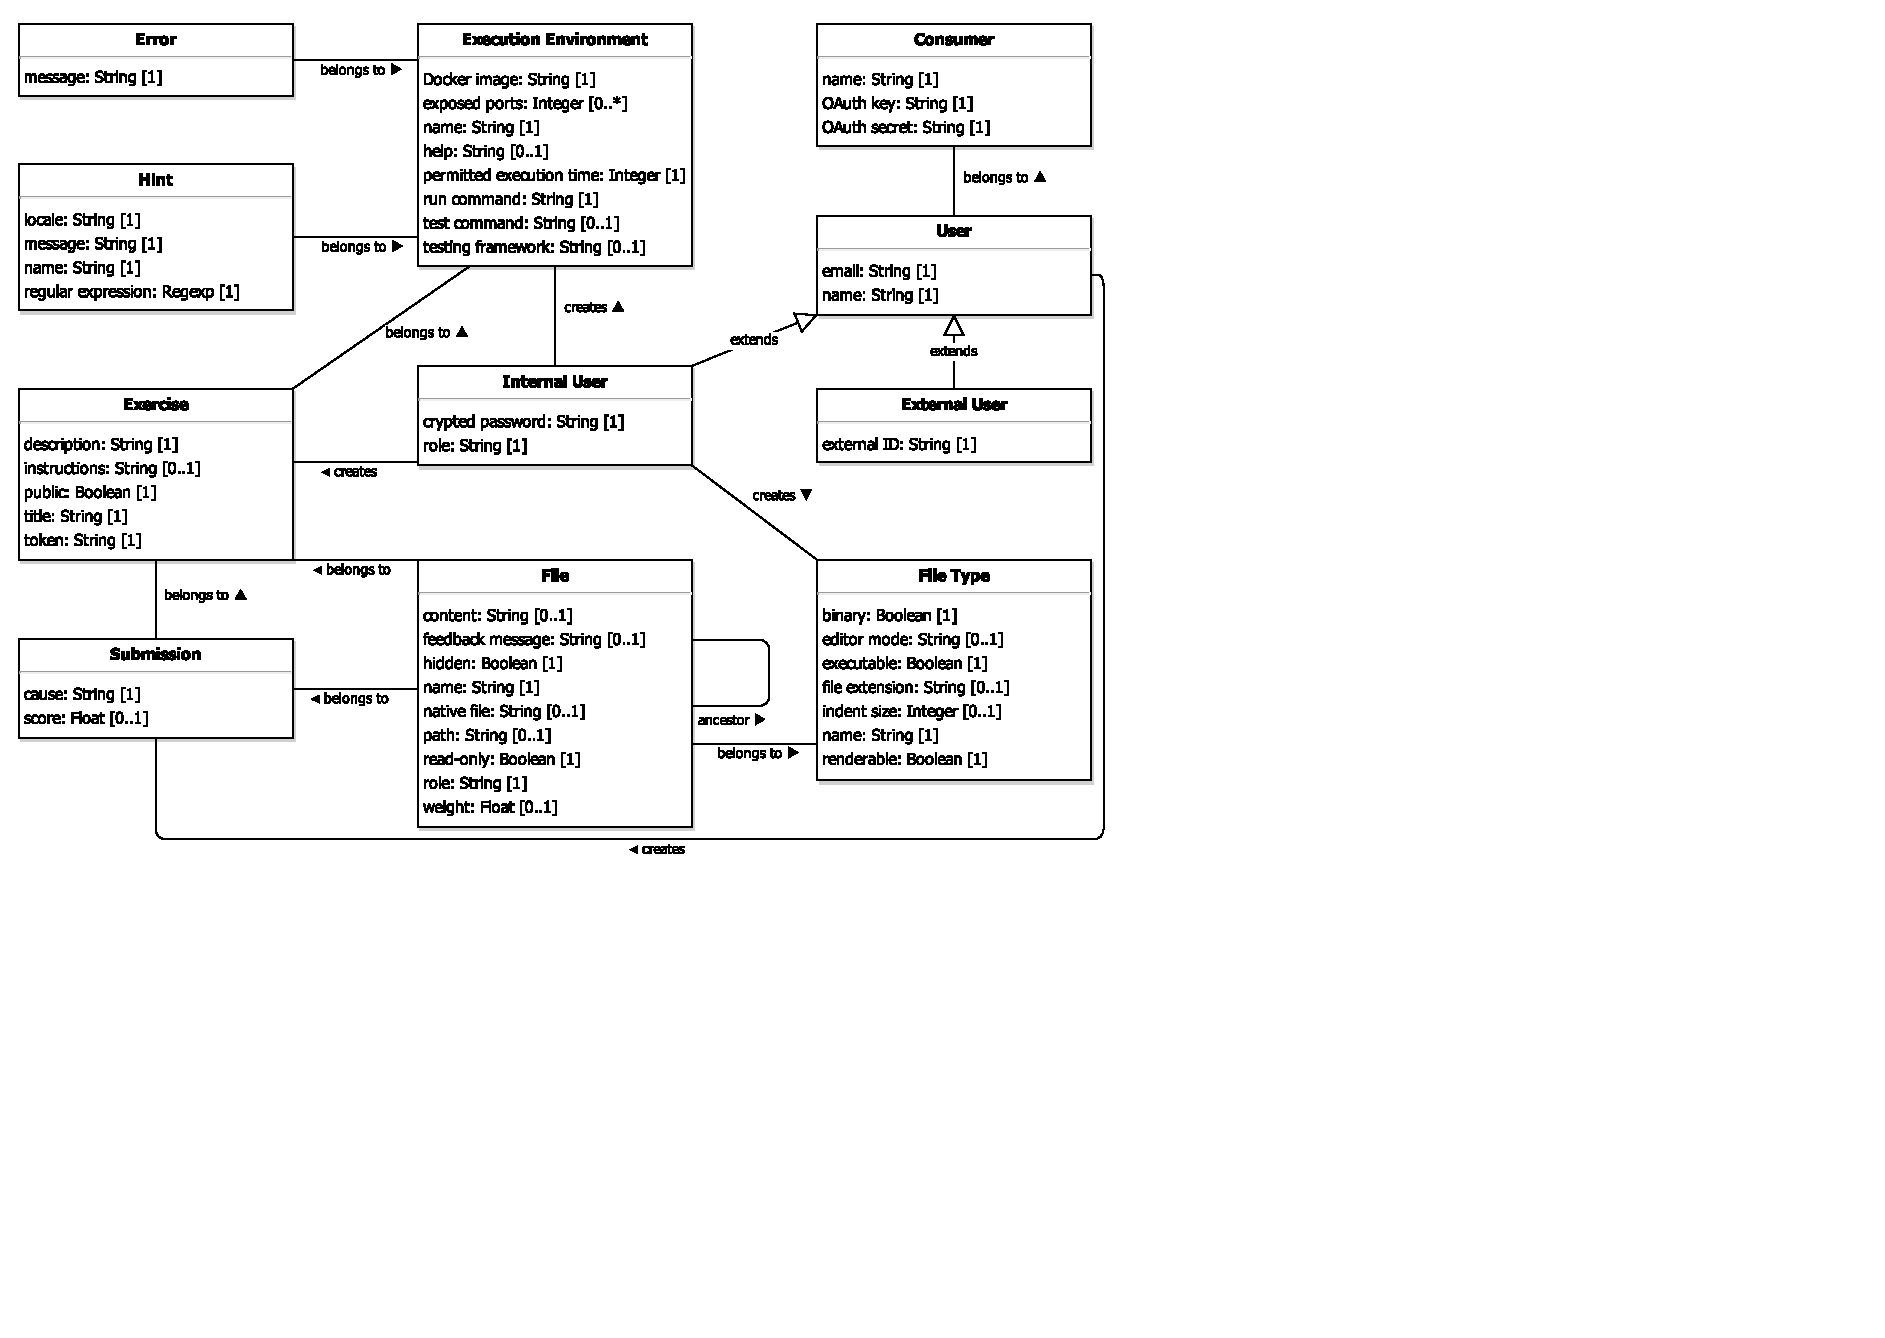
\includegraphics[clip=true, trim=0.3cm 8.1cm 13.2cm 0.3cm, width=\textwidth]{images/domain-model1.pdf}
\caption{\gls{uml} Class Diagram Presenting the Application’s Domain Model}
\label{figure:domain-model1}
\end{figure}

\subsubsection{Consumer}

As addressed in Section~\ref{section:interoperability1}, \tool provides its services to trusted e-learning applications, so-called consumers. Consumers have to be registered with \tool and have to be provided with credentials. Every consumer is assigned a name, a unique OAuth key, and an OAuth secret.

\subsubsection{User}

We identified three types of users of \tool:

\begin{itemize}
\item
  Administrators, who manage consumer applications and platform users.
\item
  Teachers, who create content, examine learners' performance, and provide hints.
\item
  Learners, who solve programming exercises.
\end{itemize}

These three user types fall into two different categories:

\begin{itemize}
\item
  Internal users, who are registered with \tool and have privileges to perform content management.
\item
  External users, who are mere visitors sent from a consumer application.
\end{itemize}

We decided to introduce two separate models for these conceptually different user classes. Moreover, since both user classes' sets of attributes are different and, more notably, their expected numbers vary significantly, we decided to store internal and external users in separate database tables instead of relying on single table inheritance~\cite{ambler2000mapping}, which is Rails' default strategy for mapping inheritance to relational databases.

Common to both user classes is that their instances belong to a consumer and have an email address and a name. While internal users provide this information in the registration process, external users' attributes are collected from the data provided during the launch of an \gls{lti} session.

\paragraph{Internal User}

Internal users have to sign in to \tool using email address and password. Therefore, every internal user has an encrypted password. Additionally, each internal user has a role, which is either \emph{administrator} or \emph{teacher}.

\paragraph{External User}

In addition to the attributes shared with internal users, external users have an external \gls{id} that is provided by the associated consumer.

\subsubsection{Execution Environment}

An execution environment describes a software platform used for the execution of code submissions. For instance, custom execution environments can be prepared for the requirements of individual courses, course modules, and even exercises.

Every execution environment is associated to the internal user who created it. An execution environment's central element is its Docker image, which provides an \gls{os} as well as third-party applications and libraries. Depending on the execution environment's needs, the permitted execution time for student-written code and a number of exposed ports can be specified. An execution environment's run command is necessary for executing code on behalf of a learner. In addition, its test command and testing framework are required for executing code for the purpose of assessment. In order to supply learners with a manual or with troubleshooting information, a help text can be provided.

\subsubsection{Exercise}

Every exercise is created by an internal user and belongs to an execution environment. The exercise's creator can decide whether it is public, and therefore visible to other internal users, or not. An exercise has a title, a short description, and explicit instructions, which should be as precise and unambiguous as possible. Every exercise has a uniquely generated token that is used for referencing the exercise when embedded by means of \gls{lti}. The core of an exercise is a collection of files, which may comprise skeleton code, tests, a reference solution, media, auxiliary scripts, and more.

\subsubsection{Submission}

A submission is a snapshot of a user's ongoing implementation of an exercise. For the main part, it consists of a number of files, which are either skeleton files that were modified or custom student-created files. Every submission has a cause, which refers to the reason why it was created.

Submissions are either created explicitly on behalf of a user or implicitly when saving code is a precondition for code execution. Submissions are created explicitly when a user saves her current progress or submits a finished implementation for grading. Submissions are created implicitly whenever custom files are added or deleted, before code is run for exploration, and before code is run for assessment.

Lastly, a submission can have a score, which is only true for submissions created for assessment.

\subsubsection{File}

As mentioned above, files exist either as part of an exercise or as part of a submission. A file that belongs to a submission and that is a modification of an instructor-provided file keeps a reference to this file, which is its ancestor.

Every file has a name and a file type. The content of a binary file is stored using a native file system file, whereas a non-binary file's content is stored in the database. A file's path refers to its path in the exercise workspace and can be used to realize an implicit workspace folder structure, for example to reflect the package structure in a Java project. A file's role is needed for detecting an exercise's main file, for collecting all test cases for assessment, and for setting up \gls{ui} controls for file-related operations. During exercise creation, instructors can decide if a file is visible for learners, hidden from learners, or viewable in read-only mode.

Two further attributes exist that are only relevant for files containing test cases. A test file's weight equals the score that is awarded when all contained tests are passed. A test file's feedback message is displayed to the user when at least one test fails.

\subsubsection{File Type}

File types are created by instructors corresponding to the files they want to represent in their exercises.

Every file type has an editor mode and an indent size, which control associated files' visual properties when displayed in \tool's editor. Binary attributes indicate whether files of a certain type are binary, executable, or renderable in a web browser. A file type's file extension is used for file system operations and for presenting files in the \gls{ui}.

\subsubsection{Hint}

As introduced in Section~\ref{section:hint-generation1}, \tool provides hints that facilitate beginners' understanding of programming mistakes.

Every hint belongs to a specific execution environment. A hint's regular expression is used for matching the errors that it refers to. A hint has a locale, which allows generating its message in the learner's preferred language.

\subsubsection{Error}

\enlargethispage{\baselineskip}

Errors that occur during the execution of learners' code are stored and aggregated in order to provide teachers with a guideline towards their students' common misconceptions.

Besides an association to an execution environment, errors comprise their original message.
